\chapter{Fundamentação teórica}

\section{Conceitos fundamentais}

\subsection{Definição de combustão e estequiometria}
De acordo com Turns (2013, p. 9), a combustão pode ser descrita como "[...] a oxidação rápida gerando calor, ou ambos, calor e luz; também, a oxidação lenta acompanhada por pequena liberação de calor e sem emissão de luz". Uma definição alternativa é proposta por Rendeiro et al. (2008, p. 29), que define combustão como "[...] uma reação química exotérmica entre um combustível e um comburente, usualmente o oxigênio, para liberar calor e formando como produto um grupo de espécies diferente dos reagentes". 

Um processo de combustão é dito estequiométrico quando a quantidade de oxidante fornecida é exatamente a necessária para promover a combustão completa de certa quantidade de combustível \cite{Turns}. De modo geral, os combustíveis usados em reações de combustão são hidrocarbonetos, e o agente oxidante é o oxigênio. Todavia, a combustão com oxigênio puro só se justifica em casos específicos devido ao alto custo de separar o oxigênio do nitrogênio no ar atmosférico, de forma que a combustão usualmente é modelada considerando a reação ocorrendo com ar atmosférico, composto de aproximadamente 21\% de $\ch{O2}$ e 79\% de $\ch{N2}$ \cite{Amazonia}. Para esse caso, a reação de combustão estequiométrica de um hidrocarboneto genérico $\ch{C}_x \ch{H}_y$ pode ser descrita pela Equação molecular \eqref{eq:combest}.
\begin{equation} \label{eq:combest}
\ch{C}_x \ch{H}_y + a_t(\ch{O2} + 3,76 \ch{N2}) \rightarrow{} x \ch{CO2} + y \ch{H2O} + w \ch{N2}.
\end{equation}

A presença do nitrogênio na reação permite que a temperatura da chama, e consequentemente dos gases de combustão, seja reduzida, evitando danos estruturais aos reatores. Todavia, a altas temperaturas ocorre a dissociação do nitrogênio, o que propicia a formação de $\ch{NO}$, produto prejudicial do ponto de vista ambiental \cite{Amazonia}, como será discutido posteriormente. O princípio da conservação da massa torna possível inferir, da Equação \eqref{eq:combest}, que
\begin{equation}
a_t = x + y/2.
\end{equation}

Esse equilíbrio permite definir um parâmetro chamado fração combustível-ar, Equação \eqref{eq:AF}:
\begin{equation} \label{eq:AF}
F = \left(\frac{F}{A}\right) = \frac{m_f}{m_a} 
\end{equation}

\noindent onde $m_a$ indica a massa de ar e $m_f$ indica a massa de combustível (do inglês \textit{fuel}). No caso da estequiometria a proporção é comumente indicada por $\left(\frac{F}{A}\right)_{s}$ (o subscrito s deriva do inglês \textit{stoichiometric}).
Costa (2020, p. 24) ressalta que "cada combustível possui uma quantidade estequiométrica de oxidante, que pode ser determinada através do balanço de massa atômico entre reagentes e produtos da combustão". Dessa forma, a primeira tarefa ao se avaliar um processo de combustão é determinar a quantidade estequiométrica de oxidante.

Ao se tratar de reações químicas, é importante definir parâmetros relacionados à quantidade de matéria. Um deles é a fração mássica de uma espécie química, que para uma espécie química genérica $i$ é definida pela Equação \eqref{eq:y} \cite{Turns}. Os termos $m_i$ e $m_{tot}$ se referem à massa da espécie química e à massa da mistura, respectivamente.
\begin{equation} \label{eq:y}
Y_{i} = \frac{m_i}{m_{tot}} \left[\frac{kg}{kg_{mistura}}\right].
\end{equation}

A fração molar é definida semelhantemente, dessa vez em função do número de mols da espécie química e da mistura ($N_i$ e $N_{tot}$, respectivamente), como mostra a Equação \eqref{eq:cai}.
\begin{equation} \label{eq:cai}
\chi_{i} = \frac{N_i}{N_{tot}} \left[\frac{kmol}{kmol_{mistura}}\right].
\end{equation}

\subsection{Razão de equivalência}
O modelo estequiométrico de um processo de combustão é o ponto de partida para sua análise; todavia, na maioria das aplicações práticas a proporção de oxidante fornecida ao processo é diferente da estequiométrica. Caso a quantidade de oxidante fornecida à reação seja maior do que a estequiométrica, a mistura é dita pobre em combustível. Analogamente, caso essa quantidade seja menor, a reação é dita rica em combustível \cite{Turns}. Quantitativamente, essa característica é expressa através da razão de equivalência ($\Phi$), definida na Equação \eqref{eq:phi} em função da fração combustível-ar estequiométrica ($F_s)$ e modificada ($F$).
\begin{equation} \label{eq:phi}
\Phi = \frac{F}{F_{s}} .
\end{equation}

Da equação acima constata-se que caso $\Phi > 1$ a mistura é rica, para $\Phi < 1$ a mistura é pobre, e para $\Phi = 1$ a proporção é a estequiométrica. Uma grandeza equivalente à razão de equivalência é o excesso de ar ($\%e$), Equação \eqref{eq:excess}, que indica, em porcentagem, o quanto de ar adicional é inserido no processo.
\begin{equation} \label{eq:excess}
\%e = \left(\frac{1-\Phi}{\Phi}\right)\cdot 100\%.
\end{equation}

Em processos de combustão, buscando-se garantir que todo o combustível seja consumido, os reagentes são usados com misturas pobres (Rendeiro et al. (2008) propõe como referência 3\% de excesso de oxigênio, ou seja, 15\% de excesso de ar). Já em processos distintos, como a gaseificação, onde os produtos desejados são principalmente $\ch{CO}$ e $\ch{H_2}$, o processo ocorre com excesso de combustível, operando com apenas 30\% da quantidade de ar estequiométrica \cite{Amazonia}. Especialmente se o processo desejado for a pirólise, que consiste no aquecimento de um material em atmosfera pobre em oxigênio a fim de se obterem combustíveis sólidos, líquidos ou gasosos, $\Phi$ deve ser muito alto.

\subsection{Entalpia de combustão e poderes caloríficos}
A entalpia de combustão pode ser definida como a diferença entre a entalpia dos produtos e a entalpia dos reagentes quando um processo de combustão completa ocorre a uma temperatura e pressão dadas \cite{Shapiro}. Ou seja, é numericamente igual ao calor liberado por um reator no qual ocorre um processo de combustão completo onde os produtos estão à mesma pressão e temperatura que os reagentes. É dada em função das entalpias dos produtos e dos reagentes da reação ($h_{prod}$ e $h_{reag}$, respectivamente):
\begin{equation} \label{eq:entcomb}
\Delta h_R = h_{prod} - h_{reag}.
\end{equation}

\noindent Tendo em vista que $h_{prod}$ é menor que $h_{reag}$, a entalpia de combustão é um valor negativo, e usualmente é dada em $kJ/kg_{comb}$.

O poder calorífico de um combustível é o valor em módulo da entalpia de combustão \cite{Shapiro}. Essa métrica indica a máxima quantidade de calor possível de ser extraída de uma certa massa de combustível. O poder calorífico superior (PCS) é o calor de combustão calculado supondo que a água proveniente da reação foi condensada; já o poder calorífico inferior (PCI) supõe que a água esteja no estado gasoso após a combustão \cite{Turns}. Como a condensação da água é um processo exotérmico, mais energia estará disponível, o que torna o PCS numericamente superior ao PCI. Entretanto, usualmente é o PCI que é usado para a caracterização do combustível.

A partir do PCI é possível definir a potência de um processo de combustão cujo fornecimento de combustível seja constante, a uma vazão mássica $\dot{m}_{comb}$, Equação \eqref{eq:Pot}:
\begin{equation} \label{eq:Pot}
P = \dot{m}_{comb} \cdot PCI.    
\end{equation}


\subsection{Eficiências associadas a processos de combustão}
A eficiência térmica é definida como sendo a razão entre a energia pretendida e a energia gasta. Considerando um processo de combustão, esta eficiência pode ser definida através da Equação \eqref{eq:efcomb} \cite{Turns}. O termo $\dot{Q}_{comb}$ indica o calor disponível na reação e $\dot{m}_{comb}$ é a vazão mássica de combustível.
\begin{equation} \label{eq:efcomb}
\eta_{c} = \frac{\dot{Q}_{comb}}{\dot{m}_{comb}\cdot PCI},
\end{equation}

A eficiência de combustão também pode ser definida em termos de outros parâmetros. Kirch et al. (2018), por exemplo, definem uma eficiência de combustão nominal, em termos de parâmetros relacionados a emissões de poluentes, frequentemente usada no caso de reatores de massa fixa empregados domesticamente. Essa eficiência, chamada pelos autores de NCE (\textit{nominal combustion efficiency}) é definida na Equação \eqref{eq:efcombn}, onde $\chi_{\ch{CO2}}$ e $\chi_{\ch{CO}}$ são as frações molares de dióxido e monóxido de carbono, respectivamente. 
\begin{equation} \label{eq:efcombn}
NCE = \frac{\chi_{\ch{CO2}}}{\chi_{\ch{CO2}} + \chi_{\ch{CO}}},
\end{equation}

\subsection{Biomassa e formação de poluentes}
A biomassa pode ser definida como um material de origem orgânica no estado vivo ou morto, bem como seus respectivos produtos e resíduos \cite{Spliethoff}. Se trata de uma fonte de energia renovável, tendo em vista que sua reposição pela natureza é muito mais rápida do que seu consumo \cite{Brand}. A biomassa a ser tratada no presente trabalho é a florestal, proveniente de resíduos de madeira proveniente de reflorestamento, que posteriormente passam por um processo de peletização.

Em termos de composição, comumente a biomassa lignocelulósica apresenta os elementos C, H, O, N e S (embora a presença de enxofre usualmente é tão baixa que pode ser desprezada). Dessa forma, o processo de combustão estequiométrico apresentado na Equação  \eqref{eq:combest} para a biomassa é melhor descrito através da Equação química \eqref{eq:combestbio}. Os coeficientes da reação química são determinados com base em um balanço de massa. 
\begin{equation} \label{eq:combestbio}
\ch{C} \ch{H}_a \ch{O}_b \ch{N}_c \ch{S}_d + a_t(\ch{O2} + 3,76 \ch{N2}) \rightarrow{} x \ch{CO2} + y \ch{H2O} + z \ch{SO2} + w \ch{N2}.
\end{equation}

No caso de uma reação com excesso ou falta de ar, os produtos da combustão variam, sendo formados compostos intermediários tais como $\ch{CO}$, $\ch{SO_{x}}$ ($\ch{SO} + \ch{SO2}$), $\ch{NO_{x}}$ ($\ch{NO} + \ch{NO2}$), hidrocarbonetos (principalmente $\ch{CH4}$, $\ch{C2H4}$, $\ch{C2H6}$), dentre outros em mais baixa concentração \cite{Lora}. Essa variação pode ocorrer inclusive em uma combustão estequiométrica, tendo em vista que, na prática, a distribuição de ar e combustível não é uniforme dentro do reator. Os poluentes são usualmente classificados em três categorias \cite{Amazonia}:
\begin{enumerate}[noitemsep,nosep,labelindent=\parindent,leftmargin=*,label={\alph*}) ] 
	\item gases que provocam efeito estufa: $\ch{CO2}$ e hidrocarbonetos;
	\item gases nocivos à saúde: $\ch{CO}$, $\ch{SO_{x}}$, $\ch{NO_{x}}$;
	\item resíduos inertes: carbono fixo residual e cinzas.
\end{enumerate}

Dentre os citados acima, os poluentes mais prejudiciais são os produtos que contêm enxofre e nitrogênio. Compostos sulfurados, além de promoverem corrosão superficial dos equipamentos, dão origem à chuva ácida caso sejam lançados na atmosfera. Já os nitrogenados também podem originar chuva ácida, e ao reagirem com o oxigênio produzem ozônio (\ch{O3}), prejudicial em baixas altitudes \cite{Amazonia}. O monóxido de carbono (\ch{CO}) é nocivo à saúde humana tendo em vista que, ao se combinar com a hemoglobina do sangue, impede a absorção de oxigênio, o que pode levar inclusive à morte.

Como já mencionado, tipicamente a biomassa lignocelulósica possui teores de enxofre tão baixos que usualmente sua presença é desprezada. Todavia, a presença de nitrogênio muitas vezes é relevante, como será visto a seguir. Nesse contexto, diversos autores investigam maneiras mais eficazes de converter a biomassa em energia, combinando diferentes processos a fim de maximizar a energia produzida mantendo a emissão de poluentes mínima. No presente trabalho a ênfase é dada em reatores que combinam gaseificação e queima, cujas emissões de $\ch{CO}$, material particulado e $\ch{NO_{x}}$ são reduzidas \cite{Kirch2018}.

%%%%%%%%%%%%%%%%%%%%%%%%%%%%%%%%%%%%%%%%%%%%%%%%%%%%%%%%%%%%%%%%%%%%%%%%%%%%
\section{Processos para conversão da biomassa em energia}
A biomassa pode ser convertida em energia de variadas maneiras, sendo os processos mais empregados a conversão térmica, bio-química e química. Dentre os processos térmicos, ganham destaque a gaseificação e a pirólise; os processos bio-químicos são a fermentação e digestão anaeróbia; e como processo somente químico é destacada a transesterificação \cite{Singh}. A Figura \ref{fig:Pic_biomass} mostra de maneira concisa os referidos processos.

\begin{figure}[!ht]
	\centering
	\caption{Processos de conversão de biomassa em energia.}
	\frame{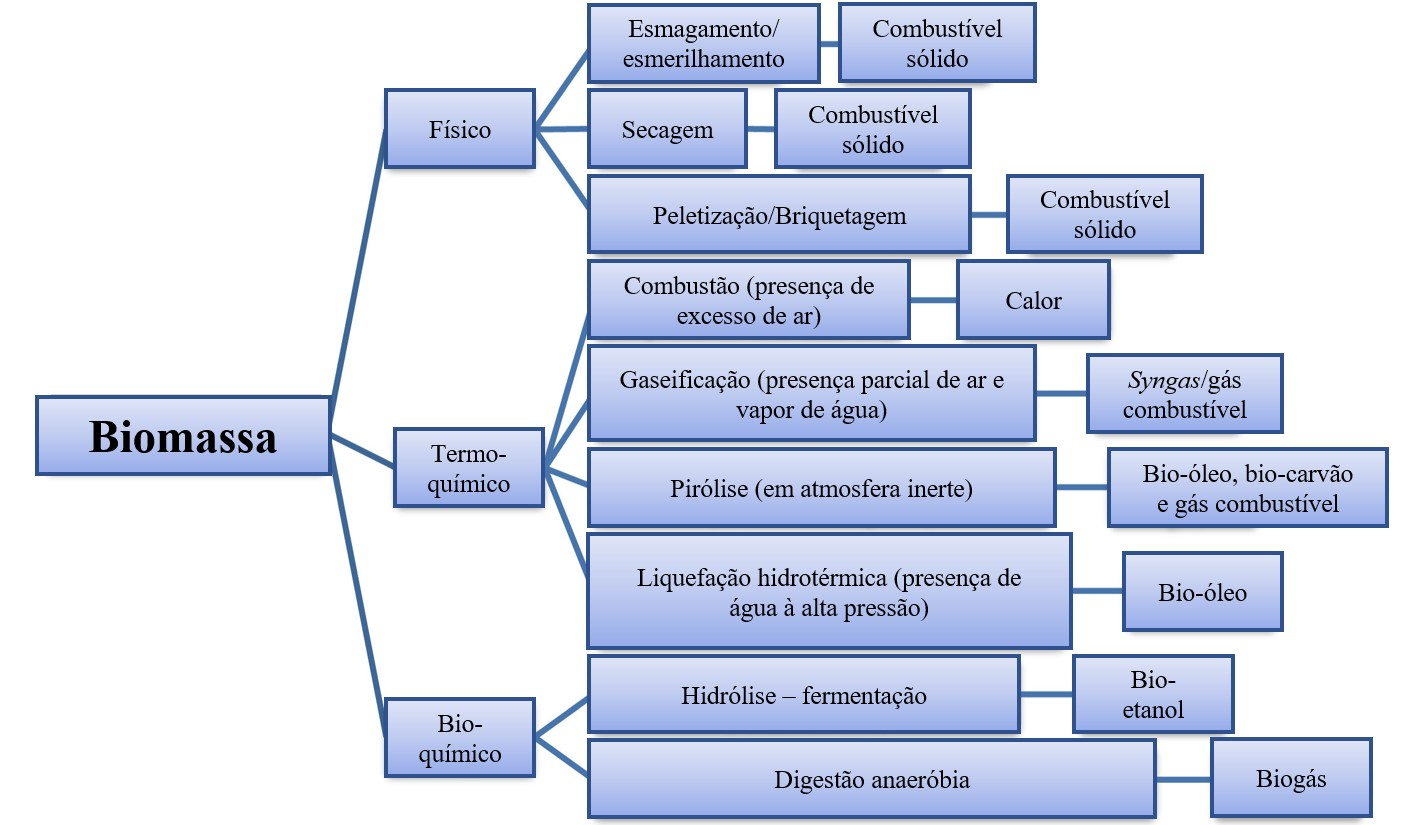
\includegraphics[scale=0.35]{Textuais/Pic_biomass.jpg}}
	\fonte{Adaptado de Sharma, Pareek, Zhang (2015).}
	\label{fig:Pic_biomass}
\end{figure}

A seguir serão apresentados e discutidos os processos térmicos e a queima direta. 

\subsection{Queima direta}
A queima direta, ou incineração, consiste no processo de combustão com a presença de ar em excesso. Para a queima direta da biomassa são necessários grandes volumes de ar atmosférico, e os produtos da reação são basicamente gás carbônico e vapor de água. A energia liberada no processo é o produto de interesse, podendo ser usada para a geração de vapor, que movimentará turbinas e permitirá a geração de energia elétrica \cite{Kretti}, ou somente a fim de produzir calor.

Nos processos de combustão de biomassa, podem ser formadas pequenas quantidades de monóxido de carbono, hidrocarbonetos e demais gases não desejados, tendo em vista que parte do carbono e hidrogênio não reagem completamente com o oxigênio \cite{Brand}. O processo também gera resíduos na forma de cinzas, que não participam da combustão, ainda que no caso de pellets de madeira o teor de cinzas seja geralmente baixo \cite{Spliethoff}. A decomposição da biomassa no caso da combustão se dá em uma sequência de etapas, sendo elas a secagem, pirólise/gaseificação, ignição dos voláteis e combustão do carbono fixo \cite{Brand}.

Dentre os processos térmicos para produção de energia elétrica por meio da biomassa, a combustão é um processo comercial já consolidado, diferentemente da gaseificação, que ainda espera por uma aceitação do mercado como uma possibilidade de produção de biocombustíveis sintéticos \cite{Neves2017}. Por outro lado, muitas vezes o alto teor de umidade da biomassa bruta prejudica a estabilidade da combustão, sendo necessário o estudo de outros processos de conversão ou tratamentos para a biomassa anteriores à combustão \cite{Yaman2004}.

\subsection{Pirólise}
A pirólise é definida por Singh et al. (2010, p. 1373, tradução nossa) como "mudanças químicas que ocorrem quando calor é aplicado a um material na ausência de oxigênio". É um processo que não somente pode ser aplicado à biomassa, mas a diversos outros materiais, a fim de gerar energia. A pirólise é um dos poucos processos que permite que um combustível líquido seja produzido a partir da biomassa \cite{Basu}.

De maneira geral a pirólise de um hidrocarboneto genérico pode ser descrita pela Equação química \eqref{eq:pirolise}:
\begin{equation} \label{eq:pirolise}
\ch{C}_n \ch{H}_m \ch{O}_p + calor \rightarrow{} \sum_{liquido} \ch{C}_a \ch{H}_b \ch{O}_c + \sum_{gas} \ch{C}_x \ch{H}_y \ch{O}_z + \sum_{solido} \ch{C}
\end{equation}

Os produtos da pirólise da biomassa são um sólido de alto teor de carbono, conhecido como coque (ou bio-carvão, ou ainda carbono fixo), e uma fração de voláteis (gases e vapores). Os vapores podem ser condensados gerando um líquido conhecido como bio-óleo ou líquido pirolenhoso, composto de ácido acético, metanol, alcatrão solúvel e insolúvel, etc. \cite{Brand}. Esse líquido pode ser armazenado e usado para produção de energia; já o gás resultante pode ser usado para fornecer energia ao próprio reator \cite{Sharma2015}. É composto principalmente por gases não condensáveis, como $\ch{CO2}, \ch{CO}, \ch{N2}, \ch{H2}$ e hidrocarbonetos \cite{Brand}. 

Os produtos resultantes da pirólise da biomassa dependem da maneira como o processo ocorre. Por exemplo, no caso da pirólise rápida a alta temperatura, o produto em maior quantidade será gás; em contraponto, caso deseje-se maior teor de líquidos, o processo deve ocorrer a menores temperaturas, com alta taxa de fornecimento de calor e com baixo tempo de residência de gás no processo \cite{Singh}. De acordo com Di Blasi apud Sharma et al. (2015, p. 1083, tradução nossa), "Um dos benefícios significativos da pirólise é que é possível conduzi-la em temperaturas mais baixas (normalmente no intervalo de 673-973 K) do que as requeridas nos processos de gaseificação (> 973 K) e combustão (> 1173 K)".

\subsection{Gaseificação}

A gaseificação é constituída por uma série de etapas sequenciais que buscam transformar a nível termoquímico um material sólido ou líquido em um gás sintético. O produto resultante é um gás composto predominantemente por $\ch{H2}$, CO, $\ch{CO2}$, $\ch{N2}$, $\ch{CH4}$ e, em menor quantidade, hidrocarbonetos e demais contaminantes \cite{Nagafugi}, sendo referido usualmente na literatura como gás de síntese, ou \textit{syngas}. O processo ocorre na presença de um agente gaseificante, que pode ser ar, oxigênio, vapor de água ou uma mistura desses componentes, a altas temperaturas (entre 500 e 1400°C); pode também ser realizado a pressão atmosférica ou a altas pressões (até 33 bar). O nível de oxigênio do ambiente é baixo durante o processo, fator que limita a formação de compostos nitrogenados e sulfurados, $\ch{NO}_x$ e $\ch{SO}_x$ respectivamente \cite{Ismail2019}.

O gás resultante no processo pode ser usado diretamente como combustível, sendo oxidado no próprio reator ou armazenado para processo posterior, ou servir de matéria prima para a síntese de produtos químicos. Duas alternativas são possíveis para a biomassa: gaseificá-la diretamente ou convertê-la em carvão vegetal e gaseificar o carvão, sendo que cada um possui vantagens e desvantagens \cite{Brand}.

Em termos de processo, quatro etapas principais ocorrem em reatores de gaseificação, sendo elas a secagem, pirólise, combustão e redução. Na secagem ocorre a evaporação da água contida no combustível (umidade) devido ao aumento da temperatura. A pirólise é a fase em que os gases inflamáveis contidos no sólido são liberados, mediante alta temperatura, sendo que esses gases se misturam com o oxigênio do ar para formar misturas inflamáveis. A combustão é a reação do carbono com o oxigênio, sendo esse um processo exotérmico cuja principal função é fornecer energia para os demais processos ocorrerem. A redução é o processo de gaseificação propriamente dito, onde o carbono sólido se transforma em carbono gasoso através de reações endotérmicas \cite{Amazonia}. A zona onde cada reação ocorre depende do tipo de gaseificador que está sendo usado \cite{Kretti}, sendo que a classificação dos reatores será abordada posteriormente nesse trabalho.

As reações de redução do carbono (quando inicialmente na forma de carvão vegetal) são mostradas nas Equações moleculares abaixo:
\begin{gather} 
	\ch{C} + \ch{CO2} \rightarrow{} 2\ch{CO}   \label{eq:gas1};  \\
	\ch{C} + \ch{H2O} \rightarrow{} 2\ch{CO} + \ch{H2} \label{eq:gas2}; \\
	\ch{C} + 2\ch{H2} \rightarrow{} \ch{CH4} \label{eq:gas3}; \\
	\ch{CH4} + 2\ch{H2O} \rightarrow{} \ch{CO} + 3\ch{H2O} \label{eq:gas4}.
\end{gather}

Barata (2014) ressalta que a gaseificação apresenta-se como um processo mais limpo, tendo em vista que os sólidos residuais do processo (principalmente as cinzas) permanecem dentro do reator, o que diminui a emissão de particulados. Entretanto, para que o gás possa atender aos requisitos de uso, ele deve ser tratado adequadamente. Por exemplo, para uso em turbinas e sistemas de geração de eletricidade, o gás deve estar livre de particulados, alcatrão, compostos de enxofre, cloro e de metais alcalinos. Constitui exceção o caso em que os gases gerados são queimados em sistemas acoplados de gaseificação-combustão, no qual não é necessário tratamento \cite{Brand}. De modo geral, a eficiência do processo é bem alta; se analisada a eficiência como sendo a energia dos gases gerados em relação ao conteúdo da matéria prima, valores típicos obtidos são de 80 a 85\% \cite{Brand}.

Basu (2010, p. 70, tradução nossa) enfatiza que a pirólise "não possui qualquer similaridade com o processo de gaseificação, este envolvendo reações químicas com um agente gaseificante externo conhecido como meio de gaseificação". Os processos diferem também em termos da temperatura, sendo que a pirólise tipicamente ocorre em uma faixa de 300 a 650°C, enquanto a gaseificação ocorre entre 800 e 1000°C \cite{Basu}.

%%%%%%%%%%%%%%%%%%%%%%%%%%%%%%%%%%%%%%%%%%%%%%%%%%%%%%%%%%%%%%%%%%%%%%%%%%%%
\section{Composição e caracterização da biomassa}
Na biomassa lignocelulósica, proveniente da madeira, plantas e folhas, as três macromoléculas em maior quantidades são a hemicelulose, celulose e lignina, sendo que as duas primeiras formam as fibras de madeira e a última mantêm as fibras juntas \cite{Amazonia}. Além de carbono, hidrogênio, oxigênio e nitrogênio, também são encontrados na biomassa resquícios de cálcio, potássio, silício, magnésio, alumínio, enxofre, dentre outros \cite{Febrero2015}. Uma das vantagens da biomassa lignocelulósica é que, diferentemente do amido ou dos carboidratos, a celulose não participa da dieta humana, e seu uso portanto não ameaça a produção de alimentos para consumo humano \cite{Basu}.

Um dos parâmetros fundamentais relativos a biomassa é o teor de umidade ($\omega_{bu}$), que expressa a massa de água contida na biomassa ($m_{\ch{H2O}}$), podendo ser definido pela Equação \eqref{eq:baseumida} no caso de base úmida (quando a massa de água é incluída na massa total, denotada por \textit{bu}). Na Equação, $m_{bio seca}$ se refere à massa de biomassa seca.
\begin{equation} \label{eq:baseumida}
\omega_{bu} = \frac{m_{\ch{H2O}}}{m_{\ch{H2O}}+m_{bio seca}}.
\end{equation}

\noindent Essa quantia pode também ser expressa em base seca (bs), ou seja, o termo $m_{\ch{H2O}}$ é nulo no denominador da Equação \eqref{eq:baseumida}. A título de comparação, o teor de umidade para toras de madeira deixadas ao tempo é de 40 a 55\% bu , já para madeiras secas esse teor cai para uma faixa de 8 a 12\% bu. Sena (2021, p. 18) ressalta que "quanto menor o teor de umidade, maior é a produção de calor por unidade de massa". Entretanto, um teor de umidade inferior a 8\% bu é prejudicial à estrutura da biomassa, pois nesse caso inicia-se um processo de decomposição das estruturas moleculares da madeira \cite{Amazonia}. Além disso, uma biomassa com teor de umidade muito baixo torna o processo de peletização mais difícil, pois propicia uma queima superficial indesejada \cite{Sena2021}.

Outro parâmetro relevante na caracterização da biomassa é a massa específica. Quando se trata de biomassa não contínua, como é o caso de pellets de madeira, é mais conveniente definir uma massa específica aparente (também chamada de densidade a granel, Equação \eqref{eq:rho}). V denota o volume do recipiente usado para determinação do parâmetro. 
\begin{equation} \label{eq:rho}
\omega_{\rho_{ap}} = \frac{m_{biomassa}}{V}.
\end{equation}

\noindent Essa medida é dita aparente pois existem espaços não preenchidos entre os pellets, tornando a medida menor do que a massa específica real \cite{Amazonia}. A massa específica aparente é um parâmetro muito relacionado à logística, pois quanto maior essa propriedade, mais quantidade de massa pode ser transportada em um mesmo volume, tornando o processo mais viável economicamente \cite{Sena2021}.

Algumas características da biomassa são determinadas com base na chamada análise imediata, sendo elas o teor de voláteis, cinzas e carbono fixo \cite{Basu}. O teor de materiais voláteis é definido como a quantidade de componentes que podem ser removidos por efeito somente da temperatura em atmosfera inerte ou não oxidante \cite{Sena2021}. O teor de voláteis na biomassa de madeira é geralmente alto, variando entre 76 e 86\% bs \cite{Obernberger2004}. Já o teor de cinzas quantifica a quantidade de resíduos sólidos que sobram após a queima completa do combustível. As cinzas são compostas principalmente de óxidos minerais, e também fazem parte da sua composição possíveis resquícios de poeira, terra etc. \cite{Sena2021}. Obernberger et al. (2004) cita que, para biomassa de madeira densificada, o teor de cinzas geralmente situa-se entre 0,4 e 1,3\% bs. 

A caracterização de biomassa proveniente de madeira é realizada com base nas normas da ASTM (\textit{American Society for Testing and Materials}). Vale ressaltar que a norma brasileira mais próxima para se caracterizar combustíveis de origem lignocelulósica foi a NBR 8112, usada para caracterização de carvão vegetal; todavia a norma foi cancelada no ano de 2015. As principais normas de ensaio para obtenção da análise imediata de combustíveis provenientes da madeira são relacionados por Basu (2010):
\begin{enumerate}[noitemsep,nosep,labelindent=\parindent,leftmargin=*,label={\alph*}) ] 
	\item teor de voláteis: ASTM E-872;
	\item teor de cinzas: ASTM D-1102;
	\item teor de umidade: ASTM E-871;
	\item teor de carbono fixo: obtido pela diferença. 
\end{enumerate}

Alternativamente, a análise imediata pode ser realizada através de análise termogravimétrica. Nessa técnica, uma amostra de combustível sólido é aquecida em atmosfera específica em uma microbalança eletrônica. A variação de massa do combustível, indicada por um dispositivo específico de termogravimetria, permite determinar os teores de umidade, materiais voláteis e teor de cinzas \cite{Basu}.  

A composição em termos dos elementos básicos é determinada pela análise elementar, sendo a composição do combustível então descrita em termos do teor de C, H, O, N, S, cinzas e umidade. Se trata de uma análise relativamente mais cara e complicada, se comparada à análise imediata \cite{Basu}. Basu (2010) menciona as normas ASTM E-777, E-778, E-775 para determinação do teor de carbono e hidrogênio, nitrogênio e enxofre, respectivamente, para biomassa proveniente de refugo. O teor de umidade e cinzas é determinado de acordo com as normas já mencionadas anteriormente. A Tabela \ref{tab:elementar} relaciona características de diversos tipos de biomassa, bem como suas principais propriedades. 

\begin{table}[!htbp]
	\centering
	\small
	\renewcommand{\arraystretch}{1.3}
	\caption{Composição elementar de alguns tipos de biomassa.}%
	\label{tab:elementar}
	\begin{tabular}{|l|l|l|l|l|l|l|l|}
    	\hline
        \textbf{Biomassa}    & \textbf{C (\%)} & \textbf{H (\%)} & \textbf{O (\%)} & \textbf{N (\%)} & \textbf{S (\%)} & \textbf{Cinzas (\%)} & \textbf{Fonte}      \\
        \hline
        Plátano              & 50,6            & 6,0             & 41,7            & 0,3             & 0               & 1,4                  & Basu (2010)         \\
        \hline
        Cascas de arroz      & 39,2            & 5,1             & 35,8            & 0,6             & 0,1             & 19,2                 & Basu (2010)         \\
        \hline
        Serragem             & 47,2            & 6,5             & 45,4            & 0               & 0               & 1,0                  & Basu (2010)         \\
        \hline
        Eucalipto         & 46,3±0,5        & 6,4±0,1         & 46,8±0,6        & 0,1±0,0         & -               & 0,4±0,0              & Neves et al. (2017) \\
        \hline
        Pinus             & 48,0±1,2        & 6,3±0,1         & 45,1±1,2        & 0,1±0,0         & -               & 0,5±0,0              & Neves et al. (2017) \\
        \hline
        Pellets   & 49,1±1,0        & 6,6±0,1         & 43,5±1,1        & 0,1±0,0         & -               & 0,7±0,0              & Neves et al. (2017) \\
        \hline
        
    \end{tabular}

	\vspace{2mm}
	\fonte{O autor.}
\end{table}

%Outra propriedade que permite caracterizar a biomassa é o PCI. Os fatores que mais influenciam o poder calorífico da biomassa lignocelulósica são a composição química, tipo, teor de umidade e teor de cinzas. Brand (2010) destaca que espécies de plantas gimnospermas (coníferas) de maneira geral possuem poder calorífico maior do que angiospermas. Um maior teor de umidade também implica em um menor poder calorífico líquido; da mesma forma, quanto maior o teor de cinzas, menor é o PCI, tendo em vista que as cinzas não participam das reações \cite{Brand}. 

\subsection{Peletização}
Dentre os processos de adensamento da biomassa lignocelulósica, um dos mais importantes é a peletização (do inglês \textit{pelletization}). O processo permite o aumento da densidade energética do combustível, bem como facilita o transporte e armazenamento. Outras vantagens dos pellets são seu alto poder calorífico, fácil ignição, além de possuírem baixo teor de cinzas e enxofre \cite{Lin2021}. 

O processo de peletização é realizado através de uma prensa, que realiza pressão sobre a biomassa moída e força-a a passar sobre uma matriz com perfurações circulares. O resultado são pequenos cilindros, de diâmetro entre 5 e 15 mm e massa específica que geralmente se situa na faixa de 1000 e 1300 kg/m³ \cite{Amazonia}. Geralmente não é necessária a adição dos chamados ligantes, pois a própria lignina passa por um processo de plasticização ao ser submetida às temperaturas da peletizadora, atuando então como um aglutinante natural \cite{Sena2021}.

\subsection{Efeitos de composição}
%O poder calorífico da biomassa é bastante relacionado à sua composição, bem como o modo de densificação utilizado (peletização, briquetes etc.) \cite{Spliethoff}. O mesmo autor indica o valor de poder calorífico de pellets de palha como sendo 14,4 MJ/kg. 
Os fatores que mais influenciam o poder calorífico da biomassa lignocelulósica são a composição química, tipo, teor de umidade e teor de cinzas. Brand (2010) destaca que espécies de plantas gimnospermas (coníferas) de maneira geral possuem poder calorífico maior do que angiospermas. Um maior teor de umidade também implica em um menor poder calorífico líquido; da mesma forma, quanto maior o teor de cinzas, menor é o PCI, tendo em vista que as cinzas não participam das reações \cite{Brand}. Spliethoff (2010) traz um gráfico que relaciona o poder calorífico inferior de alguns tipos de biomassa como função do teor de umidade, mostrado na Figura \ref{fig:PCIw}. O autor também cita que o PCI da biomassa lignocelulósica seca e sem cinzas situa-se na faixa entre 17 e 21 MJ/kg.
\begin{figure}
	\centering
	\caption{PCI como função da umidade para palha (\textit{straw}) e madeira (\textit{wood}).}
	\frame{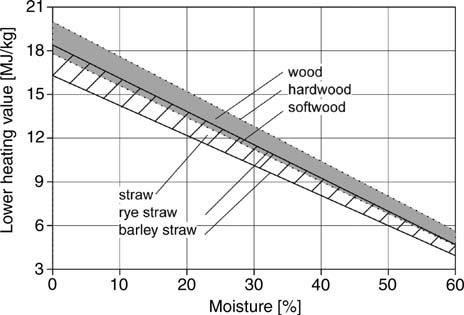
\includegraphics[scale=0.7]{Textuais/Pictures/moistureLHV.png}}
	\fonte{Spliethoff (2010).}
	\label{fig:PCIw}
\end{figure}

Outro ponto em que a biomassa se diferencia em relação aos combustíveis tradicionais, tal como o carvão mineral, é o teor de voláteis. A Figura \ref{fig:volatiles} mostra um gráfico que relaciona o teor de voláteis (\textit{volatiles}), cinzas (\textit{ash}) e carbono fixo (\textit{coke}) para dois tipos de carvão, palha e madeira.

\begin{figure}
	\centering
	\caption{Teores de voláteis, cinzas e carbono fixo para diferentes combustíveis sólidos.}
	\frame{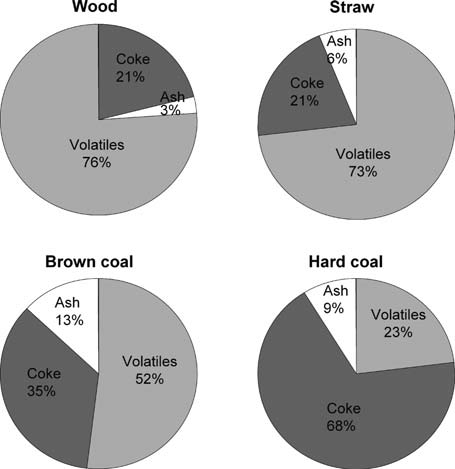
\includegraphics[scale=0.7]{Textuais/Pictures/volatiles.png}}
	\fonte{Spliethoff (2010).}
	\label{fig:volatiles}
\end{figure}

Em relação a composição dos voláteis emitidos pela biomassa, existem diversos estudos, com enfoque principalmente na gaseificação. Neves et al. (2017) avaliam a composição dos voláteis gerados no processo de gaseificação de quatro tipos de pellets em um reator de leito fluidizado. Os testes foram conduzidos para uma faixa de temperatura de 600 a 975°C, sendo a temperatura média do leito 750°C. Os autores mediram a concentração dos gases formados na pirólise em função da temperatura, usando o balanço de massa para verificar a consistência dos dados. Os gases avaliados como produtos da pirólise foram $\ch{H2}, \ch{CO}, \ch{CO2}, \ch{CH4}, \ch{C2H4}$ e $\ch{C2H6}$, sendo $\ch{C3H8}$ também verificado como um produto relevante. Uma das principais conclusões é que a composição do gás resultante é bastante correlacionada à temperatura do processo, sendo que a produção de $\ch{H2}$ e $\ch{CO}$ tem um aumento acentuado com o aumento da temperatura, enquanto para os demais gases verifica-se um pico de produção em uma temperatura intermediária. Essa dependência é semelhante em todos os quatro tipos de pellets testados, à exceção da produção de $\ch{CO}$, que varia conforme o teor de oxigênio do combustível. 

Por fim, outro fator relevante em termos da composição da biomassa é a possibilidade de formação de incrustações no reator. Febrero et al. (2015) analisaram a formação de incrustações em um modelo de pequena escala de um queimador de pellets. Dois elementos críticos nesse aspecto foram o cloro e enxofre, sendo que no caso do combustível em questão o cloro foi o elemento que mais formou incrustações nas superfícies de troca de calor. Os demais elementos residuais analisados permaneceram junto às cinzas, sendo mais facilmente removidos do processo. O estudo também concluiu que o volume de ar injetado no reator deve ser o maior possível, quando o objetivo é evitar incrustações.

\section{Reatores para biomassa}
Dentre os tipos de reatores para processamento de biomassa, ganham destaque os gaseificadores, que proporcionam a formação do gás combustível necessário para o processo de queima. A Figura \ref{fig:gasification_technologies} apresenta um panorama das principais tecnologias de gaseificação.

\begin{figure}[!ht]
	\centering
	\caption{Tecnologias de gaseificação.}
	\frame{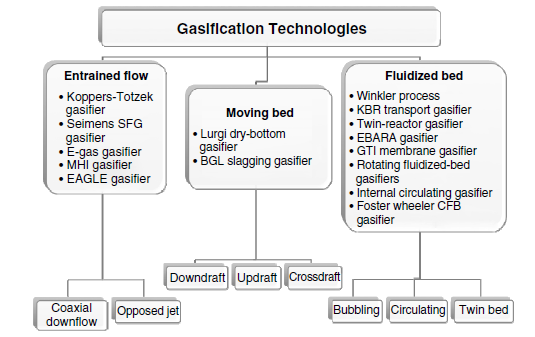
\includegraphics[scale=0.7]{Textuais/gasification_technologies.png}}
	\fonte{Basu (2010).}
	\label{fig:gasification_technologies}
\end{figure}

Ainda, os reatores podem ser classificados de acordo com a alimentação de biomassa, sendo tipos possíveis os de alimentação contínua, intermitente ou por lote (encontrado na literatura como \textit{batch}, onde toda a biomassa é adicionada no início do processo) \cite{Kruger}. Em reatores de combustão para biomassa de leito fixo, como os voláteis se desprendem e são queimados sobre o leito, é conveniente dividir o fluxo de ar em duas partes, um fluxo para a combustão do carbono fixo e outro para a combustão dos voláteis. O objetivo nesse caso é promover a queima completa dos voláteis e do carbono fixo \cite{Brand}.

O reator do presente trabalho se encaixa na categoria \textit{moving bed}, no qual existe uma grade que suporta a biomassa, e o combustível desce conforme vai sendo consumido \cite{Basu}. Essa categoria por sua vez se divide em três outros tipos: \textit{updraft} (contracorrente), \textit{downdraft} (co-corrente), e \textit{crossdraft} (corrente cruzada). A seguir serão detalhados os reatores contracorrente, co-corrente e os reatores multi-estágios, que aliam o processo de volatilização (gaseificação ou pirólise) ao de queima em um mesmo equipamento.

\subsection{Reatores contracorrente}
Nesse tipo de reator o meio de gaseificação, que geralmente é o ar, é inserido pelo fundo do reator e ascende em direção ao topo, enquanto o combustível se move para baixo \cite{Basu}. Uma representação é dada na Figura \ref{fig:updraft}.

\begin{figure}[!ht]
	\centering
	\caption{Esquema de reator do tipo contracorrente, com as principais reações e distribuição de temperaturas.}
	\frame{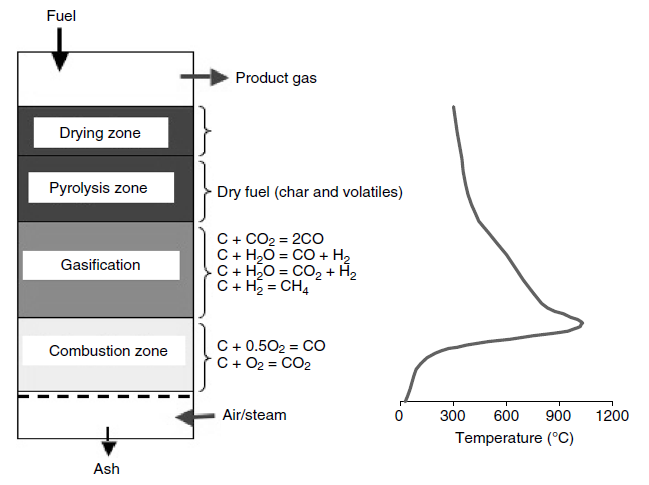
\includegraphics[scale=0.6]{Textuais/updraft.png}}
	\fonte{Basu (2010).}
	\label{fig:updraft}
\end{figure}

Se trata de um reator adequado para biomassa com alto teor de cinzas (até 25\%) e umidade (60\%). São verificadas altas taxas de formação de alcatrão, tornando o reator menos adequado para combustíveis com alto teor de voláteis. Entretanto, é possível queimar o gás logo após sua produção, o que promove a participação do alcatrão na reação. Nesse caso, não é necessária a limpeza do gás, e o uso de combustíveis com teor de voláteis mais alto não se torna um problema \cite{Basu}.

\subsection{Reatores co-corrente}
Diferentemente dos reatores contracorrente, nesse caso o agente gaseificador é inserido apenas na metade do reator e os gases resultantes do processo são retirados pelo fundo. Um esquema desse tipo de reator é mostrado na Figura \ref{fig:downdraft}.

\begin{figure}[!ht]
	\centering
	\caption{Reator do tipo co-corrente.}
	\frame{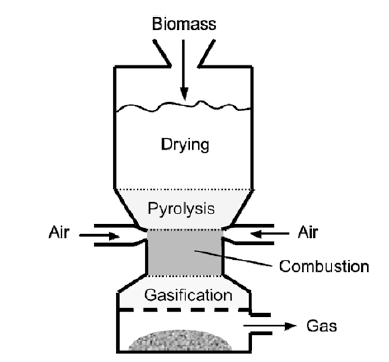
\includegraphics[scale=0.6]{Textuais/downdraft.png}}
	\fonte{Basu (2010).}
	\label{fig:downdraft}
\end{figure}

Primeiramente ocorre a evaporação da água presente na biomassa, e em seguida, sob o efeito do calor produzido na zona de reação e sem existência de oxigênio, ocorre a pirólise. O ar somente é introduzido na metade do reator, onde então ocorre a combustão. Por fim, o gás resultante (produtos da combustão + oxigênio) é direcionado pela camada de carbono fixo formada, gaseificando-a. Os gases podem ser retirados então pelo fundo do reator \cite{Basu}.

Uma das vantagens de um reator desse tipo é o fato de que os gases produzidos passam próximo à camada de cinzas na base, o que favorece reações de craqueamento do alcatrão, gerando um produto com baixo teor desse elemento \cite{Basu}. Esse fator faz com que o gás gerado no processo possa ser diretamente usado em um motor de combustão interna, por exemplo.

%\subsection{Reatores Crossdraft}
%Ver se é necessário falar.

\subsection{Queimador multi-estágios}
Nesse caso o gás gerado no processo de gaseificação é queimado logo após sua formação. Uma das vantagens desse processo é a redução de custos, caso o produto desejado seja somente calor, tendo em vista que o gás combustível produzido por gaseificadores contracorrente possui alto teor de alcatrão. Dessa forma, é necessário um processo de limpeza antes de o gás ser usado em motores ou turbinas, por exemplo. Promovendo a combustão desse gás logo após sua formação, essa limpeza não é necessária \cite{Scharler2011}.

Outra vantagem é em termos de emissão de poluentes. A queima do gás proveniente da gaseificação é propensa a formação de $\ch{NO}_x$, o que pode ser melhorado justamente através da queima em duas etapas \cite{Scharler2011} \cite{Kirch2018}. No mesmo contexto, uma das desvantagens de gaseificadores contracorrente é o alto teor de alcatrão do gás resultante. Todavia, quando o gás produzido é diretamente queimado, o próprio alcatrão acaba se tornando um combustível, beneficiando o processo \cite{Brunner2017}.

\subsection{Modelos de reatores da literatura}

Um modelo de reator cujo foco é unicamente a gaseificação com alimentação contínua de biomassa é proposto por Mandl et al. (2017). Nele, os autores buscam modelar matematicamente um gaseificador de leito fixo contracorrente para operação em regime permanente. Uma representação do reator, onde também são mostrados os processos aos quais os pellets são submetidos, é mostrada na Figura \ref{fig:mandl}.

\begin{figure}[!ht]
	\centering
	\caption{Modelo de gaseificador proposto pelos autores.}
	\frame{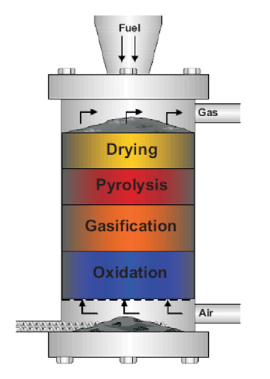
\includegraphics[scale=0.7]{Textuais/burner_mandl.png}}
	\fonte{Mandl, Obernberger, Biedermann (2010).}
	\label{fig:mandl}
\end{figure}

No topo da biomassa o processo dominante é a secagem, onde a água presente nos pellets evapora devido ao calor proveniente dos gases gerados nas etapas posteriores. Em seguida, os pellets passam pelo processo de pirólise, a uma temperatura em torno de 500 K, onde ocorre o desprendimento dos voláteis. A biomassa não volatilizada desce e, devido ao aumento da temperatura (acima de 1000 K), passa pelo processo de gaseificação. Por fim, o combustível restante no reator, que consiste basicamente em carbono fixo, é oxidado pelo ar suprido na parte inferior do reator, processo que fornece energia às demais etapas \cite{Mandl2010}.

Obernberger et al. (2017) desenvolveram um protótipo de reator onde um gaseificador de leito fixo contracorrente é diretamente acoplado a um queimador multi-estágios. O objetivo é promover um processo de baixa emissão de CO, componentes orgânicos e material particulado, tanto para combustíveis convencionais (pellets de madeira e maravalhas) quanto para os menos comuns, como resíduos florestais e resíduos provenientes da agricultura. O esquema do queimador pode ser verificado na Figura \ref{fig:obernberger}.

\begin{figure}[!ht]
	\centering
	\caption{Modelo de reator com gasificação e queima multi-estágios acoplada.}
	\frame{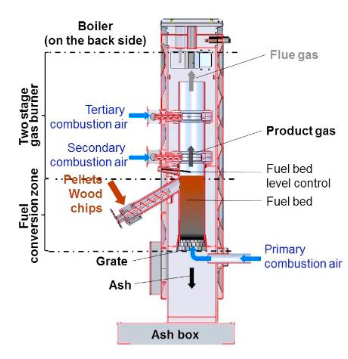
\includegraphics[scale=0.7]{Textuais/burner_obernberger.png}}
	\fonte{Obernberger et al. (2017).}
	\label{fig:obernberger}
\end{figure}

\noindent Os autores concluíram que o queimador apresenta um excelente desempenho em termos de emissão de CO e compostos orgânicos, bem como de particulados. Também foi constatado que o excesso de ar a ser utilizado pode ser baixo, da ordem de 1,2, sem ocorrência de incrustações.

Outro modelo de reator que alia gaseificação e queima é proposto por Pavel et al. (2019), mas diferentemente do anterior, esse modelo não possui alimentação contínua, sendo necessário adicionar toda a massa de combustível a ser usada no início do processo (reator do tipo \textit{batch}). Além disso, só existe uma injeção de ar na etapa de combustão. Uma representação do reator está mostrada na Figura \ref{fig:pavel}.

\begin{figure}[!ht]
	\centering
	\caption{Modelo de reator com gaseificação e queima simultâneas.}
	\frame{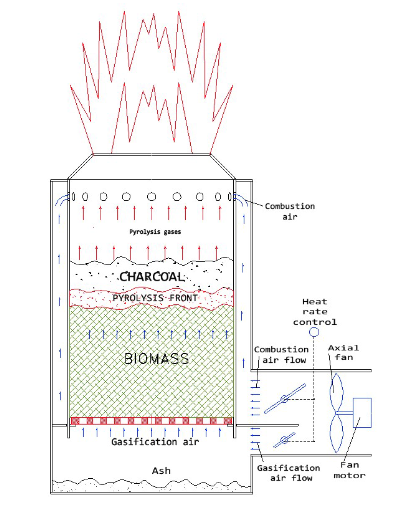
\includegraphics[scale=0.5]{Textuais/burner_pavel.png}}
	\fonte{Pavel et al. (2019).}
	\label{fig:pavel}
\end{figure}

Esse queimador possui a característica de ser do tipo \textit{top-lit}, ou seja, a ignição é feita na superfície superior da biomassa. Ocorre então a formação de uma frente de combustão, que avança em direção ao fundo do reator. O combustível próximo à zona de combustão, devido à ação da temperatura, sofre os processos de secagem e pirólise, ocorrendo então o desprendimento dos voláteis, que são direcionados ao topo do reator para serem oxidados. No momento que a frente de combustão chega ao fundo do reator, existe cerca de 10 a 20\% de carbono fixo restante, sendo esse carbono possível de ser gaseificado e queimado no topo do reator \cite{Pavel2019}.

Semelhantemente, Oberneberger et al. (2011) estudaram um gaseificador de alimentação contínua de pellets, acoplado a uma câmara separada de combustão. Os gases considerados como produtos da gaseificação são o $\ch{CO}$, $\ch{H2}$, $\ch{CO2}$, $\ch{CH4}$, além de vapor de água, nitrogênio, alcatrão e traços de hidrocarbonetos. O conjunto do reator proposto pelos autores possui ao todo três injeções de ar: a primeira injeção se situa no gaseificador, e as outras duas no queimador. A primeira injeção do queimador é dimensionada para promover uma queima pobre, a fim de proporcionar uma zona de redução, inibindo a formação de $\ch{NO}$; a segunda injeção o oxigênio restante necessário é fornecido, a fim de promover a queima completa do gás. O esquema do reator é mostrado na Figura \ref{fig:scharler}.

\begin{figure}[!ht]
	\centering
	\caption{Modelo de reator proposto por Obernberger et al. (2017)}
	\frame{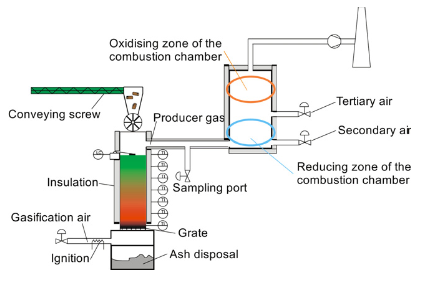
\includegraphics[scale=0.7]{Textuais/queimador_scharler.png}}
	\fonte{Mandl, Obernberger, Scharler (2011).}
	\label{fig:scharler}
\end{figure}

Nos resultados, os autores destacam que as temperaturas na base da cama de pellets (grade) chegam até 1480 K, fator que deve ser levado em conta tendo em vista a ocorrência de fusão das cinzas. Dessa forma, biomassas com ponto de fusão de cinzas muito baixo não devem ser usadas. O tipo de pirólise verificado foi a pirólise lenta, dado que foi obtido com base no tempo de residência dos pellets no reator e na temperatura alcançada. Foi verificado que o gás produzido apresenta alto teor de alcatrão, como previsto por outros autores, o que pode acarretar na condensação desse produto caso o gaseificador não seja bem isolado, especialmente em baixas vazões volumétricas de ar. Por fim, verificou-se que o modelo proposto emite pouco $\ch{CO}$, o que indica uma queima quase total do gás proveniente da gaseificação; quanto às emissões de nitrogênio, os autores verificaram que a concentração de $\ch{NO}$ não mudou significativamente ao longo da zona de redução da câmara de combustão, e que emissões de $\ch{NO}_x$ são mais baixas para uma vazão de ar menor. 

